\chapter{Structural and functional connectivity influence decision-making in communication}
\label{chap_homo}

The brain's language network has been the focus of much research relating function to underlying structure, although assessments of white matter connectivity within the language network have been rare. In this study, we examine measures from event-related functional MRI and integrate these with diffusion tensor imaging tractography and cognitive performance in 10 healthy right-handed control subjects. A communication-based decision-making task was used to identify a functional network via fMRI. Diffusion tensor tractography was used to identify the fiber tracts that provide the biological network of connections between the nodes of the functional network. Functional connectivity between regions was measured by correlating region averaged fMRI time signals and structural connectivity was measured with the average fractional anisotropy in the fiber tracts that connect the cortical regions. Stepwise multiple linear regression analysis was then used to identify the functional and structural connections that most significantly regulate cognitive performance. Both structural and functional analyses suggest that performance depends on the integration of language and decision-making subnetworks during task performance, and regression analyses suggests that measures of statistically-based functional connectivity are more sensitive than  structural connectivity at demonstrating integration within this large-scale network, but that the influence of structural connectivity is more distributed throughout the network.

%% main text
\section{Introduction}
\label{Intro}
The human brain is a system comprised of a vast number of neurons that provide great computational capacity via a complicated communication network consisting of both local circuits and long-range fiber pathways. The neurons of the cortical gray matter are responsible for processing information while the axons projecting from these neurons in the white matter provide the communication channels between the functionally and structurally segregated subregions of the cortex. The study of brain connectivity seeks to understand the interconnections, structural properties, and functional relationships of the elements of this system and is essential for further insight into the nature of complex cognitive processes supported by large-scale neural networks. In this study functional networks in the brain are examined using magnetic resonance imaging (MRI) to measure both structure and function. We hypothesize that cognitive performance will be more sensitive to the structural properties of the white matter that provides the biological network of connections than to the statistical measures of functional connectivity within the network. Tasks involving language processing and decision-making were used along with fMRI to identify the cortical regions utilized by then functional network and to allow assessment of functional connectivity between these anatomically distinct regions during performance of the tasks. Diffusion tensor imaging (DTI) was used to identify and examine the structural properties of the white matter fiber bundles that provide the communication channels between the functional regions. The network-wide measures of functional and structural connectivity were then independently used to examine their influence upon a behavioral measure of performance on the functional tasks.

\subsection{Structural Connectivity}
The set of all biological connections in the brain is known as the human connectome and provides a basis for the examination of structural connectivity~\cite{Sporns2005}. Understanding the structural connective patterns in the brain is essential to gaining further insight into the complex functional interactions that are required for complex behavior. In addition to identifying these biological connections, measuring their quality or integrity is critical to understanding the relationship between structure and function and how these together modulate behavior.  Neuroimaging techniques provide an in-vivo, macro-scale basis for a variety of methods that identify these biological connections and/or examine the structural properties of the tissues that comprise them. Studies of structural connectivity typically focus upon examining the myelinated neurons of the white matter that connect gray matter regions. In diseases that cause demyelination, anatomical images (e.g. T1- or T2-weighted images) may be used to identify white matter lesions that disrupt connectivity~\cite{Loevblad2010}. Measures of structural connectivity may also be inferred by measuring the size of white matter structures, an approach that has been used extensively to study the mid-sagittal cross-section of the corpus callosum~\cite{Witelson1989,Colcombe2005a,Gunning-Dixon2000}. 

\subsection{DTI and Structure}
Recently, the use of diffusion tensor imaging (DTI) has received a great deal of interest as a method for examining structural connectivity. DTI provides information about the orientation and micro-architecture of white matter~\cite{Basser1996}. This arises from the fact that myelin provides a barrier to the diffusion of water resulting in diffusion anisotropy where the diffusion of water is much greater along the direction of the axons than across. The orientation information provides the basis for fiber tractography methods that identify physical connections in the form of estimated white matter trajectories ~\cite{Basser2000,Mori1999a}. Measures of diffusion anisotropy, such as fractional anisotropy (FA), allow for quantitative measures of white matter integrity.  While confounded by issues such as (a) limited spatial resolution, (b) generation of false-positive connections, and (c) inability to distinguish between multiple fibers traveling in different directions within a single voxel, DTI based methods have proven useful in the examination of large, well-defined white matter fiber tracts such as the commisural fibers of the corpus callosum, the projection fibers of the thalamo-cortical network, and the association fibers of the language network. Identifying the cortical regions to which these fiber bundles extend provides the ability to examine the topography of specific white matter pathways~\cite{Behrens2003} as well as the properties of the underlying tissue. 

Following the classical anatomical teachings of connections and behavioral neurology ~\cite{Geschwind1965b,Geschwind1970}, DTI studies of living humans have demonstrated asymmetries in the left and right hemispheres of neurologically intact adults that reflect the known lateralization of language~\cite{Catani2008,Glasser2008}. Attempts have been made to relate this anatomic asymmetry to the language network. For example, an examination of the fiber tracts of the language network and demonstrated that inter-hemispheric symmetry in the arcuate fasciculus is associated with enhanced ability to remember words using semantic association ~\cite{Catani2007}. The relevance of structural connectivity to behavior was demonstrated more directly in work that found that increased FA in the white matter associated with Broca's area was higher in subjects with better grammar learning~\cite{Floel2009}. Further evidence for the behavioral relevance of FA was provided in the first study to provide evidence for white matter changes resulting from training in healthy human brain~\cite{Scholz2009}. Localized increases in FA were detected in the white matter of the intraparietal sulcus following training of a complex visuo-motor task (juggling) ~\cite{Scholz2009}. 

\subsection{Functional integration and connectivity}
Blood oxygenation level-dependent (BOLD) fMRI provides a method for measuring activation in the brain. By contrasting the activation levels associated with different experimental conditions, it is possible to identify cortical areas that are associated with specific tasks such as language processing~\cite{Frost1999,Bookheimer2002} and decision-making~\cite{Sanfey2003,McCabe2001}. To perform complex tasks, it is necessary for several anatomically distinct but functionally co-activated regions to work together and form networks under a concept known as functional integration. One way to study this integration is to examine the statistical covariance of BOLD activation in several cortical regions activated during task performance across a population~\cite{Horwitz1990,McIntosh1994}. Functional connectivity uses one of several statistical paradigms to identify coordinated activity in spatially distinct units in an individual's brain~\cite{Rykhlevskaia2008}. 

In this study, we examine the relative informativeness of functional connectivity compared to biological connectivity defined by DTI. To examine biological networks based on white matter tracts defined by DTI compared to functional connectivity defined statistically, we assessed a BOLD fMRI data set collected during an fMRI language activation study of homonyms~\cite{McMillan2010}. Briefly, this study asked subjects to make decisions about the use of a homonym or a non-homonymous synonym in a sentence. The authors hypothesized that participants would prefer to use the dominant meaning of a homonym in a context-appropriate sentence (e.g.\ ``pen" to refer to a writing implement), but would prefer to use a synonym instead of the subordinate meaning (e.g.\ ``cage" instead of ``pen" to refer to an animal enclosure). The authors demonstrated different fMRI activation patterns for each condition. A language network was recruited in the left hemisphere during stimuli with the dominant meaning, but a decision-making network was recruited additionally during subordinate stimuli. We examine the interactions between language and decision-making subnetworks using statistically-based functional connectivity and DTI-based assessments of white matter projections between activated language and decision-making regions.

\subsection{Relationship of Structure and Function}
Previous studies have attempted to combine BOLD fMRI and DTI measures in tracts between activation brain regions.
The first study to combine fMRI and DTI examined a single patient's recovery from a traumatic brain injury~\cite{Werring1998a}, and employed a converging evidence approach that relied upon qualitative analysis and formed a basis for many additional studies~\cite{Werring1999b,Jang2005,Klein2007,Munakata2006,Shinoura2006,Koch2002a}. A variety of quantitative approaches to combined analysis of DTI and BOLD fMRI have been developed. In one approach, voxelwise correlations were performed between functional and structural connectivity maps ~\cite{Olesen2003,Thomas2009}. These methods were not particularly informative because they did not heed the anatomical tracts projecting between activate regions. More recently, fMRI has been combined with DTI tractography by using functionally activated regions as seeds for tractography~\cite{Toosy2004,Powell2006,Upadhyay2007,Boorman2007,Jenkins2010}. Unless carefully constrained, this may result in the inclusion of white matter that, despite connecting to a cortical region of interest, is not part of the functional subnetwork being examined. Here we combined information from structural and functional data to restrict the analysis to fiber bundles that provide a direct biological connection between any two functional regions of interest. 

\subsection{Incorporation of Behavioral Data}
Finally, using behavioral data collected during the fMRI study as the dependent variable, we examine the relative effectiveness of statistically-based functional networks and DTI-based white matter networks to explain performance. Some previous work has related DTI and fMRI to performance. For example, Baird, et al.\ \cite{Baird2005} used reaction times and fMRI to localize cortical activity for short and long reaction times. Regression analysis using BOLD values in the activated regions as independent variables was then used to show that short reactions times were associated with FA in the splenium of the corpus callosum while long reaction times were associated with FA in the genu of the corpus callosum~\cite{Baird2005}. A study by Madden et al.\ \cite{Madden2007} combined DTI and fMRI to study the effect of aging on visual response time. Activation in the frontal and parietal cortical regions was shown to be greater for older adults, but while an age-related FA decrease was found in older adults, it did not specifically mediate the age-related changes in activation~\cite{Madden2007}. An examination of executive cognition found white matter development and age-related changes in fMRI to be directly associated with cognitive performance~\cite{Stevens2009}. Recent work by Propper et al.\ \cite{Propper2010} examining handedness and it's influence upon functional language lateralization and structure in the arcuate fasciculus suggested that degree of handedness may be an important to consider in studies of neuroanatomical asymmetries.  We hypothesize that both functional and structural connectivity may predict cognitive performance and that a stepwise multiple linear regression analysis of cognitive performance will reveal the components of the network that most influence performance. 

\section{Methods}

\subsection{Subjects}
Ten subjects (6 female) ranging in age from 19 to 32 years (mean age of 23.5 years) had both functional and diffusion tensor images. All subjects were healthy young adults participating in the study for monetary payment. All participants were native English speakers, right-handed and in good health with no history of neurological difficulty. Informed consent was obtained from all participants according to a protocol approved by the University of Pennsylvania Institutional Review Board. 

\subsection{Subnetworks in the brain} 
We investigate a hypothesis proposed by McMillan et al.\ ~\cite{McMillan2010} that suggests language processing is supported by the interaction of two cortical subnetworks, one for language and one for decision-making. This study specifically focused on the strategic process of minimizing ambiguity during language production, defined as an individuals' use of an unambiguous word (e.g.\ ``cage") instead of a semantically ambiguous word (e.g.\ ``pen") to make the meaning of an utterance more clear. A forced choice paradigm was used in which subjects were instructed to make the choice that resulted in the most clear sentence meaning (e.g.\ reduced ambiguity). 20 homonyms were identified that had a strong bias toward one of the possible meanings. The more frequent meaning (e.g.\ ``pen" is used to refer to a writing implement) is referred to as dominant while the less frequent meaning (e.g.\ ``pen" is used to refer to an animal cage) is referred to as subordinate. For each homonym, 3 context sentences were generated in which the final word was semantically related to the dominant meaning, subordinate meaning, or was semantically neutral in meaning. Additionally, a carrier sentence was generated for each homonym that consisted of a short phrase followed by a blank space. The same carrier sentence was used for dominant, subordinate, and neutral contexts for each homonym.  Lastly, a semantically related unambiguous alternative was generated. These sentences were used to create 60 experimental trials using each of the 20 homonyms in each of the contexts (dominant, subordinate, neutral). Example sentences for each condition are provided in table~\ref{sentences}~\cite{McMillan2010}. Participants were presented with a context sentence, a carrier sentence and choice between a homonym and an unambiguous alternative. To limit the participants' ability to reduce the task to homonym detection, 180 filler trials were used that followed the same format but did not include a homonym. Experimental and filler trials were randomly distributed into 5 fMRI runs of equal length. The frequency with which participants chose the unambiguous choice was recorded and used as the measure of cognitive performance.

\subsection{MRI Acquisition}
Scans were acquired on a Siemens 3.0T Trio scanner. T1-weighted structural images were acquired using an MPRAGE protocol ($TR = 1620 ms$, $TE = 3 ms$, flip angle of $15^{\circ}$, 1 mm slice thickness, $192 \times 256$ matrix, resolution = $0.9766 \times 0.9766 \times 1.0 mm$). BOLD fMRI images were acquired with fat saturation, 3 mm isotropic voxels, flip angle of $15^{\circ}$, $TR = 3 s$, $TEeff = 30 ms$ and a $64 \times 64$ matrix. DT-MRI images were acquired with 4 $b=0$ images and 30 directional diffusion weighted images (resolution = $1.875 \times 1.875 \times 2.0 mm$, $112 \times 112$ matrix, $b=1000 s/mm^2$). 

\subsection{fMRI analyses overview}
For the examination of function, the cortical regions identified by McMillan et al.\ were examined~\cite{McMillan2010}. All regions but one activated the left hemisphere. In order to limit our study to the left-hemisphere we use the left homologue to the right interior parietal region that was activated in the McMillan et al.\ study. While 18 subjects were studies by McMillan et al.\, we include only the 10 subjects for which DTI was also acquired in order to examine the relationship between function and structure. Processing of the fMRI data was performed using SPM5~\cite{SPM5}. For each subject, the functional data was motion-corrected, transformed into MNI space, spatially smoothed with a 8mm FWHM isotropic Gaussian kernel and interpolated to isotropic 2 mm voxels. A canonical hemodynamic response function was used to convolve the onset times of stimulus events for each condition. A general linear model approach was then used to calculate statistical parameter estimates for each subject. Each coordinate listed in table~\ref{PeakCoords} was used to define the center of spherical region of interest (ROI) with a 10mm radius. 

Statistically based connectivity was determined in the following manner. For each ROI in each subject, an average t-value was calculated for each context (i.e.\ dominant, neutral, subordinate). These region averaged activation values were used to examine the covariation of activation across the population via correlation analysis using Pearson's correlation coefficients. Specifically, activations corresponding to responses to each of the categories of stimuli were extracted from the fMRI time-course signal to create a time-signal with 20 time points for each context. For each ROI, the context-specific time-courses from all voxels within the ROI were used to determine an averaged time-signal for that region. These time-signals were then normalized to have a mean of 0.0 and a standard deviation of 1.0. To estimate intra-subject functional connectivity under each context, a Pearson's correlation coefficient was calculated for each region-to-region pair of interest within each subject. We limited the analysis to pairs of regions that have direct biological connections as our primary interest is in examining the relationship between structure and function and due to the limited size of the data set being examined.

\subsection{DTI analyses}
For the examination of structure, the cortical regions identified by McMillan et al.\ \cite{McMillan2010} were used to identify the white matter fiber bundles that define the biological connective network that provides communication between cortical regions. The white matter tracts of interest were identified in a diffusion tensor atlas and used to create geometric models. The models were then used to examine FA in each subject. Average FA values for each structure were calculated to provide an equidimensional framework for relating these structural measures to the functional connectivity measures that were calculated for the regions connected by each fiber tract. Specifically, we used an atlas-based methodology that provides a common anatomical frame-of-reference for inter-subject comparisons, an approach used in methods designed to identify focal white matter differences~\cite{Yushkevich2008,Goodlett2009a,Jones2002,Xu2003,Smith2006}. Fiber template were used to create arc-length parameterizations of diffusion properties due to their ability to examine whole-tract properties of white matter pathways~\cite{Jones2005,Corouge2006,Maddah2008d,Lin2006,ODonnell2009,Davis2009,Goodlett2009a,Batchelor2006}. Defining these fiber templates in the atlas space avoids the time-consuming and error-prone process of defining anatomically equivalent ROIs in each subject~\cite{Gilmore2007}. Moreover, the improved SNR provided by a population atlas provides an appropriate space for identifying fiber bundle geometry and minimizes false-positive errors~\cite{Goodlett2009a}. 

A multivariate atlas was created from a data set consisting of 30 healthy young adults for whom both high resolution T1 images and DTI were acquired. The 10 subjects from the functional study that also had DTI data were all included in this atlas-building data set. The set of all subjects' high resolution T1 weighted images were used to create an unbiased, shape averaged atlas using Symmetric Normalization as implemented in Advanced Normalization Tools (ANTS)~\cite{ANTS}. This was accomplished through the use of a multi-resolution, non-rigid registration algorithm to optimize a cross correlation metric under the constraints of a diffeomorphic transformation model~\cite{Avants2006}. The Brain Extraction Tool \cite{Smith2002} was used to segment brain parenchyma in the atlas image to create a brain mask which was propagated to each subject's T1 weighted image.  These skull-stripped T1 weighted images were then registered to the FA image derived from each subject's diffusion tensor image. The intra-subject transforms were composed with the T1 atlas transforms in order to create a subject-specific atlas with both T1-weighted and diffusion tensor data. In order to preserve the orientation information provided by the tensors, the preservation of principle technique was used along with linear interpolation of tensors in the log-Euclidean space. The T1 component of the atlas was used to determine a mapping to MNI152 space in which the functionally activated regions were defined. The use of the T1-weighted images in the atlas building was chosen because they have a higher resolution than the diffusion tensor data and to avoid using the same feature (i.e.\ FA) for registration that will later be used for statistical comparison.

The diffusion tensor component of the atlas was used to perform fiber tractography with the Camino toolkit~\cite{Cook2006}. A 1mm x 1mm x 1mm grid of points was created to fill the image space and all points in the brain with an FA of 0.2 or higher were used as seed points for deterministic tractography. The tracking proceeded from each seed point with a fixed sub-voxel step size of 0.5 mm. The local streamline direction was computed by trilinear interpolation of the eight neighboring principal directions, and tracking continued until the local FA fell below 0.15 or the streamline curved by more than 60 degrees over the length of a voxel. Landmarks were manually placed in the T1 component of the atlas in order to extract well defined white matter fiber bundles~\cite{Mori2002a,Wakana2004,Wakana2007}. The extracted fiber bundles were then used as a basis for defining a geometric model for each fiber bundle. The streamlines in each bundle were parametrized by arc-length to extend from 0.0 to 1.0. A BSpline was then fit to the arc-length parameterized streamlines in each bundle to obtain a single centerline that lies in the core of the fiber pathway of interest. For each point along the centerline, a tangent was calculated and used to determine a perpendicular plane. The intersection of this plane with each of the streamlines in the bundle defines a set of intersection points.  The normal and binormal vectors of the centerline were used to re-parameterize the intersection points into 2D coordinates. Graham's scan method was used to determine the convex hull that encloses the set of intersection points~\cite{Graham1972}, and a least-squared method was applied to the points on the hull to estimate an estimate an elliptical cross-section~\cite{Fitzgibbon1999}.

The functionally activated regions were warped into the atlas space in which tractography was performed. As white matter projections approach gray matter the fibers diverge which reduces FA and confounds fiber tractography. To account for this, the activated regions were dilated by 5mm to extend into the white matter to identify fiber bundles that provide the biological connectivity for the functional network. A fiber tract was considered to connect to a functional region if there was a non-zero overlap between the dilated cortical region and the volume enclosed by the geometric model for the fiber tract.  All fiber tracts that connect to at least two cortical ROIs are considered to be part of the biological network and are retained for examination of FA. Averaging over the full extent of white matter fiber bundles may introduce a bias due to partial voluming that occurs in voxels on the outer boundaries of the fiber tracts. We avoid this bias by incorporating a centerline or skeletonization technique that limits the examination to voxels that are near the core of the fiber tract~\cite{Smith2006,Yushkevich2008}. Here we use the centerlines provided by the geometric models to examine each subject's FA image. At each point along the centerline, FA was found. A single value was found for each fiber bundle by averaging the FA values over the length of the centerline. Tract-averaged values were chosen to reduce the problem of multiple comparisons in subsequent statistically analysis, and to provide an equidimensional basis for comparison with functional connectivity measures. We felt this was valid because the projections between activated regions must be complete in order to integrate the regions into a network.

\subsection{Relating function and structure to behavior}
Behavioral data was used to examine the extent to which functional and structural connectivity have real-world consequence regarding behavior under different contexts. To evaluate whether participants selected unambiguous alternatives at a rate that differs from random selection, the chance rate of selecting one of two responses using a binomial test was calculated. The ratio at which each subject minimized ambiguity was then used to identify the components of the networks that most directly influence performance in the functional task. To examine the relationship between performance and functional connectivity, stepwise multiple linear regression was performed using R~\cite{RStats} where the behavioral scores were the dependent variables and the functional connectivity values were the independent variables.  The initial model included functional connectivity between all regions with direct biological connections:

\begin{equation}
M^{e} = \left( \sum^{t}_{t \in S} \beta_{t}^{e} t_{FC} \right) + \epsilon
\end{equation}

where $M^{e}$ is the ratio of times in which the subject chose the word that minimized ambiguity when presented with a sentence conforming to context $e$, $S$ is the set of all white matter fiber tracts in the network, $t_{FC}$ is the functional connectivity between the cortical regions connected by fiber tract, $t$, $\beta_{t}^{e}$ is a weighting term for each connection under each condition, and $\epsilon$ is an error term. We hypothesize that performance is modulated by network-wide properties so backward elimination was used as it begins by including all components in the network. The best model was determined according to the Akaike information criterion~\cite{Akaike1974}. To examine structure, the process was repeated with the independent variables, $t_{FC}$, being replaced by $t_{FA}$, the centerline-averaged FA for a fiber tract, $t$.

\section{Results}

\subsection{Statistically-based Functional Integration and Connectivity}
A correlation analysis using Pearson's correlations was performed to examine the statistically-based strength of the relationships between the activated regions of fMRI study and how these vary under the different contexts. We found greater integration of the language and decision-making subnetworks for subordinate stimuli than dominant or neutral stimuli. The integration results are listed in Table~\ref{table:popcorrt}. In each condition, there was a statistically significant correlations between the activated regions of the language network (ATC and PLTC). The DLPFC and OFC components of the decision-making network were correlated for all conditions as well and IPC correlated with both of these regions in the subordinate context.  While many functional connections are shared by the context-specific networks, the DLPFC is particularly prominent in the subordinate context in which it significantly co-varies with all other cortical regions. The IPC also exhibits the most connections under the subordinate context. Most importantly, only 2 of 6 possible correlations were significant between the language components and the decision-making components during the dominant and neutral conditions. However, 4 of 6 correlations were statistically significant between the language and decision-making components during the subordinate condition. This emphasizes the integrated contribution of both language and decision-making components during the subordinate condition. Functional connectivity between cortical regions within individuals was examined for all pairs of regions that have a direct biological connection and are these values are summarized in~\ref{appa}. The largest and most significant functional connectivity values were found in the PLTC to DLFPC connection and the PLTC to OFC connection. 

\subsection{DTI analyses}
The functionally activated regions listed in table~\ref{PeakCoords} were used to identify the white matter tracts of interest and revealed a biological network made up of the uncinate fasciculus (UNC), arcuate fasciculus (ARC), superior longitudinal fasciculus (SLF), inferior longitudinal fasciculus (ILF), inferior frontal-occipital fasciculus (IFO) and an inferior-superior fiber bundle running along the arcuate fasciculus that will be referred to as the arcuate fasciculus vertical (AFV). The geometric models of the fiber bundles are used to define surface meshes for visualization, as illustrated in figure~\ref{fig:networkmodel}. The average FA values determined by averaging along the centerlines are summarized in~\ref{appb}. 

\subsection{Predicting Performance}
Of particular interest was the extent to which structural and functional connectivity values related to cognitive performance, how structure-specific this relationship was, and the degree to which each provided unique information. For each participant, a behavioral score was determined for each sentence context by the ratio of times that they chose the unambiguous alternative. The mean score was $0.717 \pm 0.14$. In the dominant context, participants were equally likely to choose an unambiguous alternative and homonym, while they were more likely to choose an unambiguous alternative in the neutral and subordinate contexts. 

Functional and structural connectivity values were independently examined as predictors of performance. The functional connectivity values between cortical regions for which there was a biological connection were used as independent variables in a stepwise multiple linear regression on the behavior scores. No significant results were found for the dominant and neutral contexts. For the subordinate context, the functional connectivity (Figure \ref{fig:mlr_fc}) regression analysis resulted in a model consisting of four cortical pairs($R^2=0.839, p=0.008$), including two independently significant pairs: OFC-PLTC ($p=0.005$) and OFC-ATC ($p=0.002$). To examine structural connectivity, the same analysis was performed using the averaged FA values along each fiber tract as the independent variables.  The analysis of FA also resulted in no significant results for the dominant and neutral contexts, but for the subordinate context (Figure \ref{fig:mlr_fa}) the regression analysis resulted in a model that included all fiber tracts ($R^2=0.790, p=0.074$), including four independently significant fiber tracts: AFV ($p=0.023$), IFO ($p=0.029$), UNC ($p=0.018$), and ARC ($p=0.017$).

\section{Discussion}

\subsection{Summary}
Characterizing the relationship between cognitive function and neuroanatomical structure is essential to elucidate the complex process by which the brain mediates behavior. The integration of DTI and fMRI may be an informative approach to examining this problem as it allows for non-invasive macro-scale examination of large-scale neural networks underlying behavior~\cite{Ramnani2004a,Guye2008,Rykhlevskaia2008}. Much of the recent work that combines fMRI, DTI, and behavior has focused upon examining functional activation as opposed to examining the coordinated activity between multiple activated regions as measured with functional connectivity~\cite{Aron2007a,Baird2005,Madden2007,Floel2009,Upadhyay2007}. Cohen, et al.\ ~\cite{Cohen2008a} examined how learning was influenced by both structural and functional connectivity, but with structural and functional data acquired in separate populations. Stevens, et al.\ ~\cite{Stevens2009} were the first to use fMRI and DTI to demonstrate that age related cognitive gains are associated with both white matter properties and functional integration within a network. The present study attempted to leverage multiple modern neuroimaging techniques to examine both structure and function in a young, healthy population. Specifically, the goal was to examine the utility of using fMRI and DTI to examine to gain insight into how connectivity between functional subnetworks influences real world performance in decision-making during communication. We found that language and decision-making subnetworks work together during the subordinate condition that requires the greatest dependency between these subnetworks. Additionally, we found the statistical measures of coordinated activation to be more informative than the DTI-based structural connectivity approach, but the influence of the structural properties of the neural substrates were more wide-spread in the large-scale neural network.

\subsection{Large-Scale Neural Networks}
The current work supports the theory that although specific elementary cognitive operations are localized to specific cortical regions, complex cognitive processing is achieved through the coordinated activity of multiple cortical regions to form large-scale neural networks~\cite{Mesulam1990}. A statically-based examination of functional integration demonstrated that when subjects were presented with a language-based decision, a language subnetwork was formed consisting of the ATC and PLTC, and a decision-making subnetwork was formed from the DLPFC and OFC. Increasing the difficulty required to interpret a sentence resulted in an increase in integration between the subnetworks as well as the recruitment of an additional cortical region believed to be associated with integration of subnetworks~\cite{Jaencke2001,Assmus2003}. Statical measures of functional connectivity between the cortical regions within individuals demonstrates that cognitive performance is influenced by activity throughout the network. Furthermore, a DTI-based examination of white matter structure in the fiber tracts providing the biological network that connects the cortical regions demonstrates that changes in the neural substrates of the long-range connections within in a distributed neural network~\cite{Sporns2004} directly influence cognitive performance. 

\subsection{Functional Integration}
Under all sentence conditions, significant co-activation was found within the language subnetwork (PLTC and ATC) and within the decision-making subnetwork (OFC and DLPFC). Functional integration between the subnetworks was found to vary by context. In the dominant and neutral contexts, only 2 of 6 connections between the subnetworks were found to be significant. In the subordinate context 4 of these 6 connections were significant suggesting that as sentences became more difficult to interpret, a greater integration of the language and decision-making subnetworks was required. This is supported by the connectivity of the the IPC, a region believed to be involved with integrating subnetworks. In the dominant context, the IPC had 1 significant connection of 4 possible connections and no significant connections to the IPC were found in the neutral context. However, in the subordinate context, 3 of 4 possible connections were found to be significant, including connections to components of both the language and decision-making subnetworks. This suggests that as subnetworks become integrated, it may be advantageous to recruit additional resources to facilitate communication between subnetworks.

A number of statistical methods have been proposed for examining functional integration, including principal components analysis (PCA)~\cite{Kadosh2008,Friston2000}, independent components analysis (ICA)~\cite{Greicius2007,Calhoun2008} and cross-correlation analysis (CCA)~\cite{Ma2007,Arfanakis2000}. These data-driven exploratory methods make no assumptions regarding the neuroanatomy of the underlying structural network that connects functional regions. Because we are interested in examining both the functional and biological networks, we chose to leverage a priori information about the cortical regions involved in the task and use a hypothesis-driven correlation analysis approach to examine functional integration. Model based techniques such as structural equation modeling (SEM) and dynamic causal modeling (DCM) attempt to measure the influence that one neural system has over another and have been successfully used to examine fMRI data for studies of effective connectivity. Both SEM and DCM require a priori assumptions regarding the directionality and causality of interregional influences. Here DTI-based tractography was used to identify connections between regions, but this provides a purely symmetric connection with no notion of directionality. We had no prior assumptions regarding directionality or causality within or between the subnetworks being examined, so it was appropriate to use a correlation-based method in order to avoid causal assumptions and examine what the brain is doing in contrast to model-based effective connectivity studies that seek to explicitly study how the brain is working. 

\subsection{Functional Connectivity}
Functional connectivity has been described as an `elusive concept' due to the large variety of defintions, modalities and methods that have been described using this term~\cite{Horwitz2003} so it is necessary to carefully describe exactly what this term refers to in a specific study. In this study, context-specific functional connectivity between cortical regions within an individual was measured by calculating a Pearson's correlation coefficient between region-averaged fMRI time-course signals using only the time-points that included the response to a stimuli of the given context. Under all sentence contexts, at least 90\% of subjects had significant functional connectivity between the PLTC and both components of the decision-making subnetwork (OFC and DLPFC). Examining performance in the dominant and neutral conditions with stepwise multiple linear regression analysis did not result in any significant functional connections, but in the subordinate condition it returned a model consisting of 4 connections, each including at least one component of the language subnetwork. Two functional connections were found to be independently significant, both connecting to the OFC and a language region. The OFC-ATC connections had a positive coefficient while the OFC-PLTC had a negative coefficient, possibly suggesting that the later strategy is a more effective strategy for integrating these subnetworks.

Cortical regions were identified using a priori knowledge that was used to define small ROIs over which time-signals were averaged to reduce noise in the signal. The location of these ROIs was determined in an atlas-space under the assumption that cortical activation is consistently localized between subjects. Limiting the study to these previously identified cortical regions increases the power of statistical inference~\cite{Rykhlevskaia2008}, but also prevents the identification of additional network components that may be relevant such as homologous cortical regions in the right hemisphere. The signal provided by BOLD fMRI is an indirect measure of function~\cite{Ogawa1990} and the precise nature of the relationship between the BOLD fMRI signals and the underlying neural substrate remains unknown. While there is currently no consensus on the best modality or method for examining functional connectivity~\cite{Horwitz2003}, this approach provided a statistical measure of functional connectivity that demonstrated synchronized activation within subnetworks and between subnetworks in subordinate context in which sentences are more difficult to interpret. Additionally, in the case of the subordinate context, functional connectivity values were predictive of performance.


\subsection{Structural Connectivity}
We hypothesized that structural properties of the fiber tracts that provide the communication channels between functional regions would impact the effectiveness of the network and thus influence performance. Multivariate regression analysis of tract-averaged FA throughout the biological network did not reveal any significant biological connections in the dominant or neutral context, but in the in the subordinate context the analysis resulted in a model containing all fiber tracts in the biological network. Of these tracts, 4 were found to significantly predict performance. Two of the significant fiber tracts were the IFO and the UNC each of which provides a direct biological connections between the pairs of cortical regions identified in the functional connectivity analysis (the IFO connects PTLC to ATC, and the UNC connects OFC to ATC). In both cases, the sign of the coefficient for the fiber tract matches the sign of the coefficient for the functional connectivity between the cortical regions it connects (negative for IFO and positive for UNC). Additionally, the ARC is found to be significant with a negative coefficient while the AFV is found to be significant with a positive coefficient. While the model provided by the stepwise regression analysis did not predict cognitive performance as well as the functional connectivity model, it did suggest that the influence of structure is more distributed throughout the large-scale neural network. Finding that functional connectivity is a better predictor of cognitive performance is to be expected as functional connectivity is a highly dynamic measure that is specific to the stimuli while structural connectivity in the white matter tracts that connect the functional regions is static during the presentation of the stimuli and provide connectivity for a variety of functional tasks.

The influence of white matter integrity upon performance has been examined for many specific skills and a positive correlation between FA and performance has been reported in both human~\cite{Wolbers2006,Johansen-Berg2007} and animal~\cite{Makris2007} studies, but negative correlations between FA and performance have also been reported~\cite{Tuch2005,Hoeft2007}. Studies examining the language subnetwork have reported similarly contrasting results. A positive correlation between grammar learning and FA in fiber tracts connecting to Broca's area was found in a study that used probabilistic tractography methods, resulting in a gross averaging of FA from a number of fiber tracts including the ARC, SLF, AFV, and inter-hemispheric connections through the corpus callosum~\cite{Floel2009}. A positive correlation between reading ability and FA in the temporal-parietal junction was found~\cite{Klingberg2000} and FA white matter underlying both frontal and parietal cortex was positively correlated with speed of lexical decision-making~\cite{Gold2007}. Studies examining the lateralization of the language network have also examined white matter integrity using FA. Extreme leftward lateralization in the ARC was found to be negatively correlated with verbal recall~\cite{Catani2007}. Studies including the analysis of functional data also exhibit the difficulty in interpreting FA. A positive correlation between FA in the left SLF and lateralization of fMRI based activation during verb generation has been reported~\cite{Powell2006}, as has a negative correlation between callosal FA and right prefrontal activation during verbal encoding~\cite{Putnam2008}. While these studies demonstrate that structural properties of white matter have significant influence upon behavior, they also emphasize the difficulty in interpreting FA. FA is an indirect measure of white matter integrity that is sensitive to a variety of white matter properties, including but not limited to: myelination, axon diameter and density, fiber tract curvature, and intra-voxel fiber crossings~\cite{Barkovich2000,Shimony1999,Virta1999}. FA may have a non-linear response to changes in these properties, and the relationship between FA and axon diameter is not fully known.  

An atlas-based approach was used to identify the fiber tracts allowing for the identification of well defined fiber bundles~\cite{Yushkevich2008}. This approach limits the study to easily identifiable fiber tracts as no methods exist for automatically extracting and identifying all fiber bundles in the atlas. This does not limit the current study as we are only interested in examining well defined fiber bundles that part of the accepted biological network of connections in the language and decision-making subnetworks. From the bundle of streamlines for each fiber tract, a geometric model is determined and used to identify fiber tracts that connect two cortical regions of interest. The cross-sectional areas of the fiber tracts are calculated using a least squares method and this reduces the problem of false-positive connections by limiting the influence of errant streamlines. By only examining FA along the centerline of each fiber tract, the bias caused by partial voluming is reduced as only the ``stem" of each fiber tract is examined~\cite{Smith2006,Yushkevich2008}. Additionally, averaging FA over the length of each fiber tracts should reduce the bias caused by localized fiber crossings.

\subsection{Shortcomings}
The small number of subjects limited the scope of the study, and many of the findings would not stand-up to a family-wide (FWE) error correction. A multivariate linear regression analysis examining all possible functional connections was not possible due to the small sample size and so the analysis was limited to the examination of functional connectivity between regions that were directly connected by a fiber tract identified in the DTI atlas. Additionally, the study was limited to the left hemisphere despite evidence suggesting that measures of lateralization in the language subnetwork are relevant~\cite{Catani2007,Powell2006,Putnam2008,Propper2010}. Stepwise linear regression methods has been criticized because they don't correct for multiple comparison. While this is true, we feel that multiple linear regression with backward elimination was appropriate here as we hypothesized that both functional and structural connectivity would have network-wide effects upon behavior. Additionally, the converging evidence provided by the significance of the UNC and IFO in both functional and structural analysis with corresponding coefficients strengthens our confidence in the findings. Future studies with more subjects and different task should help address these concerns.

\subsection{Conclusion}
The current study has demonstrated that both functional and structural connectivity play an critical role in modulating performance in a communication and decision-making task. The study shows that as sentences become more difficult to interpret, more integration between the language and decision-making subnetworks is required. Network-wide influences on behavior are revealed for both structural and, to a greater degree, functional connectivity. Given the relatively small population examined, future work is needed to further advance our knowledge regarding the relationship of structure and function in these brain networks. In particular, this approach may be useful in the examination of function-structure-performance relationships in a population that is hypothesized to have changes in these relationships, such as the reduced asymmetry of functional lateralization with aging~\cite{Cabeza2002}.

%


\section{Tables and Figures}
\begin{table}[h]
\begin{center}
\footnotesize{
\begin{tabular}{| l | l | l | l | l | }
\hline
{\bf Context} & {\bf Context} & {\bf Completion} & {\bf Homonym} & {\bf Alternative} \\
& {\bf Sentence} & {\bf Sentence} & {\bf Choice} & {\bf Choice}\\
\hline
Dominant & Kim had some ink. &  She needed a \_\_\_ & pen & quill\\
Subordinate & Kim had some pigs. & She needed a \_\_\_ & pen & cage\\
Neutral & Kim had some ideas. & She needed a \_\_\_ & pen & quill or cage\\
\hline
\end{tabular}
}
\caption{Example stimulus materials for the homonym ``pen" in each experimental condition. Sentences adapted from McMillan, et al.\ ~\cite{McMillan2010}}
\label{sentences}
\end{center}
\end{table}

\begin{table}[h]
\begin{center}
\begin{tabular}{| l | l l l |}
\hline
Cortical Region & \multicolumn{3}{c |}{MNI Coordinates} \\ 
\hline
Inferior parietal (IPC) & -52 & -56 & 43\\
Dorso-lateral prefrontal (DLPFC) & -48 & 23 & 36\\
Orbital frontal (OFC) & -46 & 46  & 10\\
Anterior temporal (ATC) & -48 & 15 & -16\\
Posterior lateral temporal (PLTC) & -42 & -57 & -7 \\
\hline
\end{tabular}
\caption{Peak activation MNI coordinates of functional regions of interest}
\label{PeakCoords}
\end{center}
\end{table}

\begin{table}[h]
\begin{center}
\begin{tabular}{| l | c  c  c  c |}
\hline
& DLPFC & OFC & ATC & PLTC\\
\hline
IPC & 0.318 & 0.690* & 0.558 & 0.574 \\
DLPFC & - & 0.640* & 0.732* & 0.385 \\
OFC & & - & 0.862* & 0.525 \\
ATC & & & - & 0.683* \\
\hline
\multicolumn{5}{c}{Dominant} \\
\hline
IPC & 0.519 & 0.493 & 0.279 & 0.122 \\
DLPFC & - & 0.645* & 0.582 & 0.613 \\
OFC & & - & 0.674* & 0.771* \\
ATC & &  & - & 0.720* \\
\hline
\multicolumn{5}{c}{Neutral} \\
\hline
IPC & 0.847* & 0.733* & 0.794* & 0.518 \\
DLPFC & - & 0.740* & 0.875* & 0.691* \\
OFC & & - & 0.669* & 0.448 \\
ATC & & & - & 0.641* \\
\hline
\multicolumn{5}{c}{Subordinate} \\
\end{tabular}
\caption{Population correlations of activation t-values under all conditions. * $p<0.05$. Cortical regions include orbital frontal (OFC), anterior temporal (ATC), posterior lateral temporal (PLTC), dorso-lateral prefrontal (DLFPC), and inferior partietal (IPC) }
\label{table:popcorrt}
\end{center}
\end{table}



\begin{figure}[h]
\begin{center}
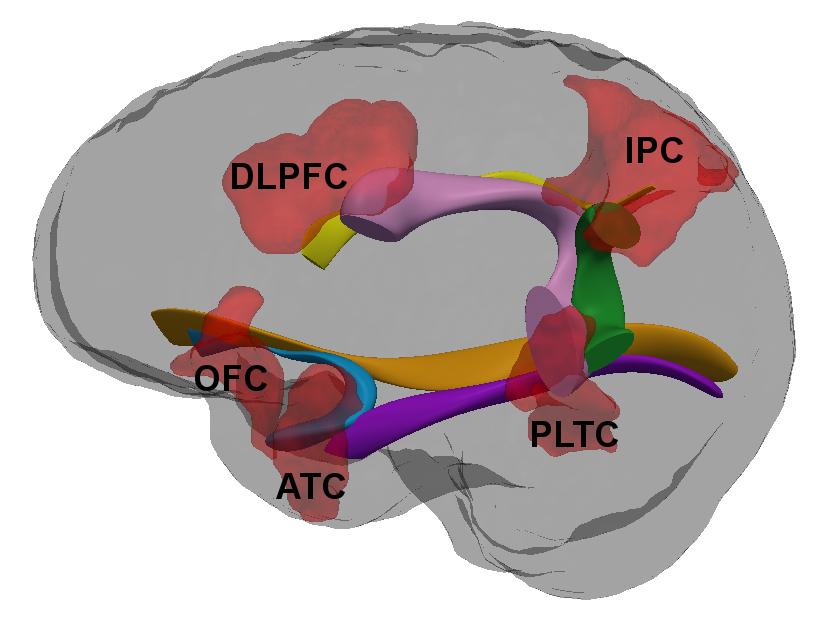
\includegraphics[width=1.0\linewidth]{figures/big_homo_labeled.png}
\caption{Functionally activated cortical regions (shown in red) were used to identify white matter fiber bundles that connected any two activated regions of interest. This resulted in the identification of the uncinate fasciculus (yellow), arcuate fasciculus (pink), inferior frontal-occiptal fasciculus (orange), inferior longitudinal fasciculus (purple), superior longitudinal fasciculus (light blue) and the arcuate fasciculus vertical (green)}
\label{fig:networkmodel}
\end{center}
\end{figure}

\begin{figure}[h]
\begin{center}
\begin{tabular}{c c}
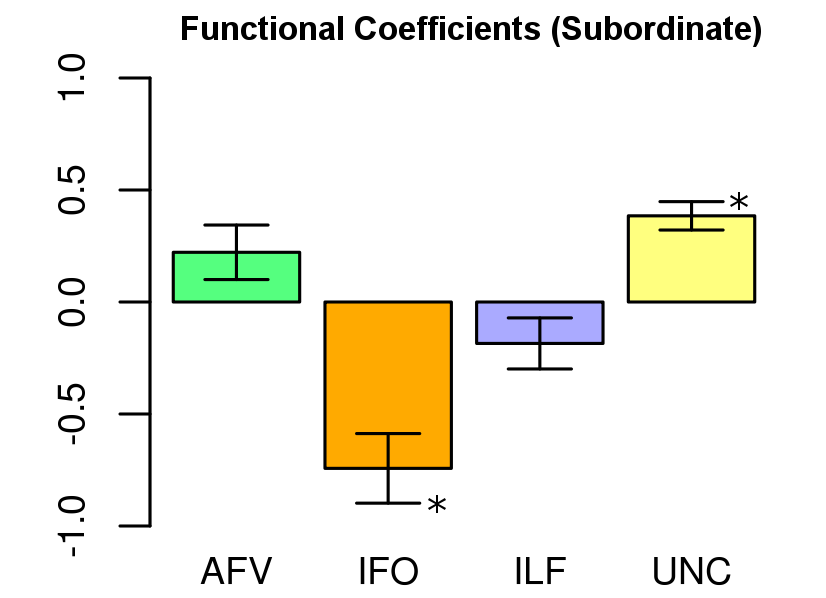
\includegraphics[width=0.45\linewidth]{figures/FC_Subordinate2.png} &
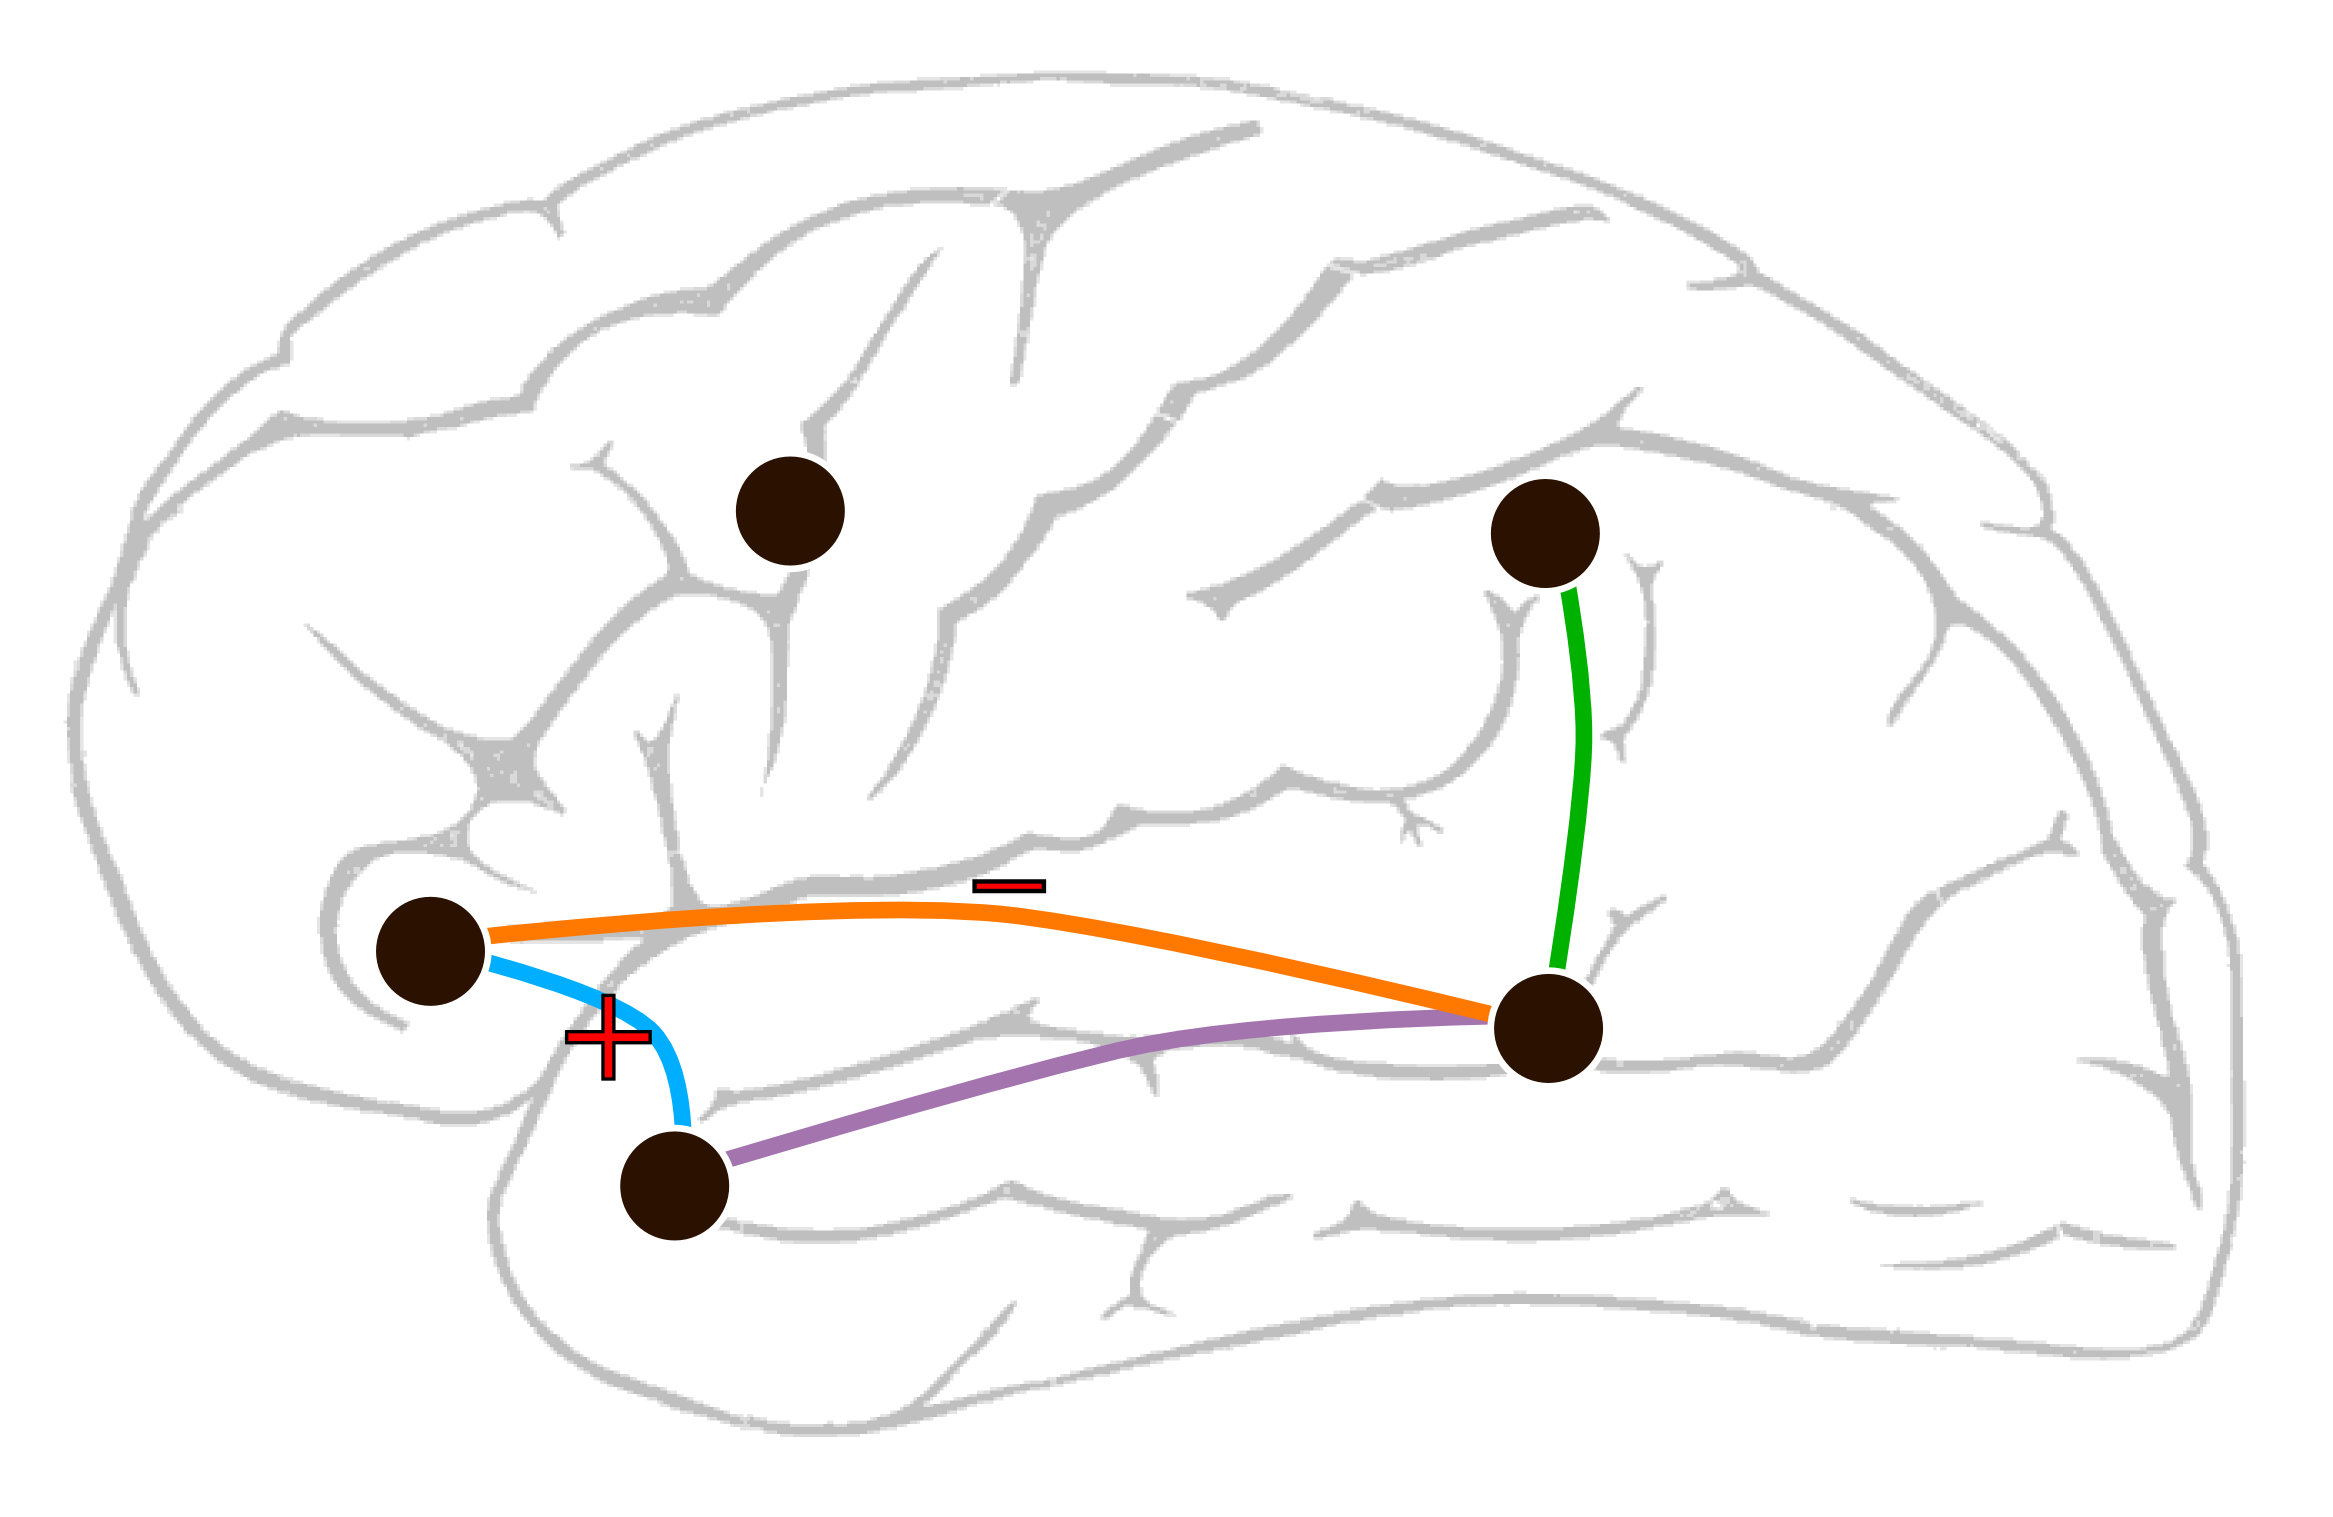
\includegraphics[width=0.45\linewidth]{figures/func_diag2.png}
\end{tabular}
\caption{Stepwise multiple linear regression analysis examining performance in the subordinate context and functional connectivity between regions connected by a white matter fiber tract resulted in a model including the vertical aspect of the arcuate fasciculus (AFV), IFO, IFL and UNC. * $p<0.05$}
\label{fig:mlr_fc}
\end{center}
\end{figure}

\begin{figure}[h]
\begin{center}
\begin{tabular}{c c}
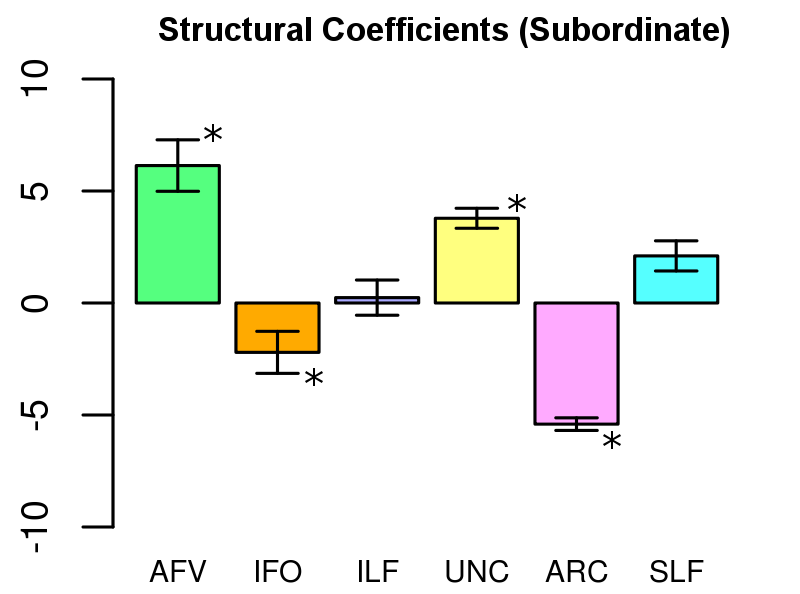
\includegraphics[width=0.45\linewidth]{figures/FA_Subordinate2.png} &
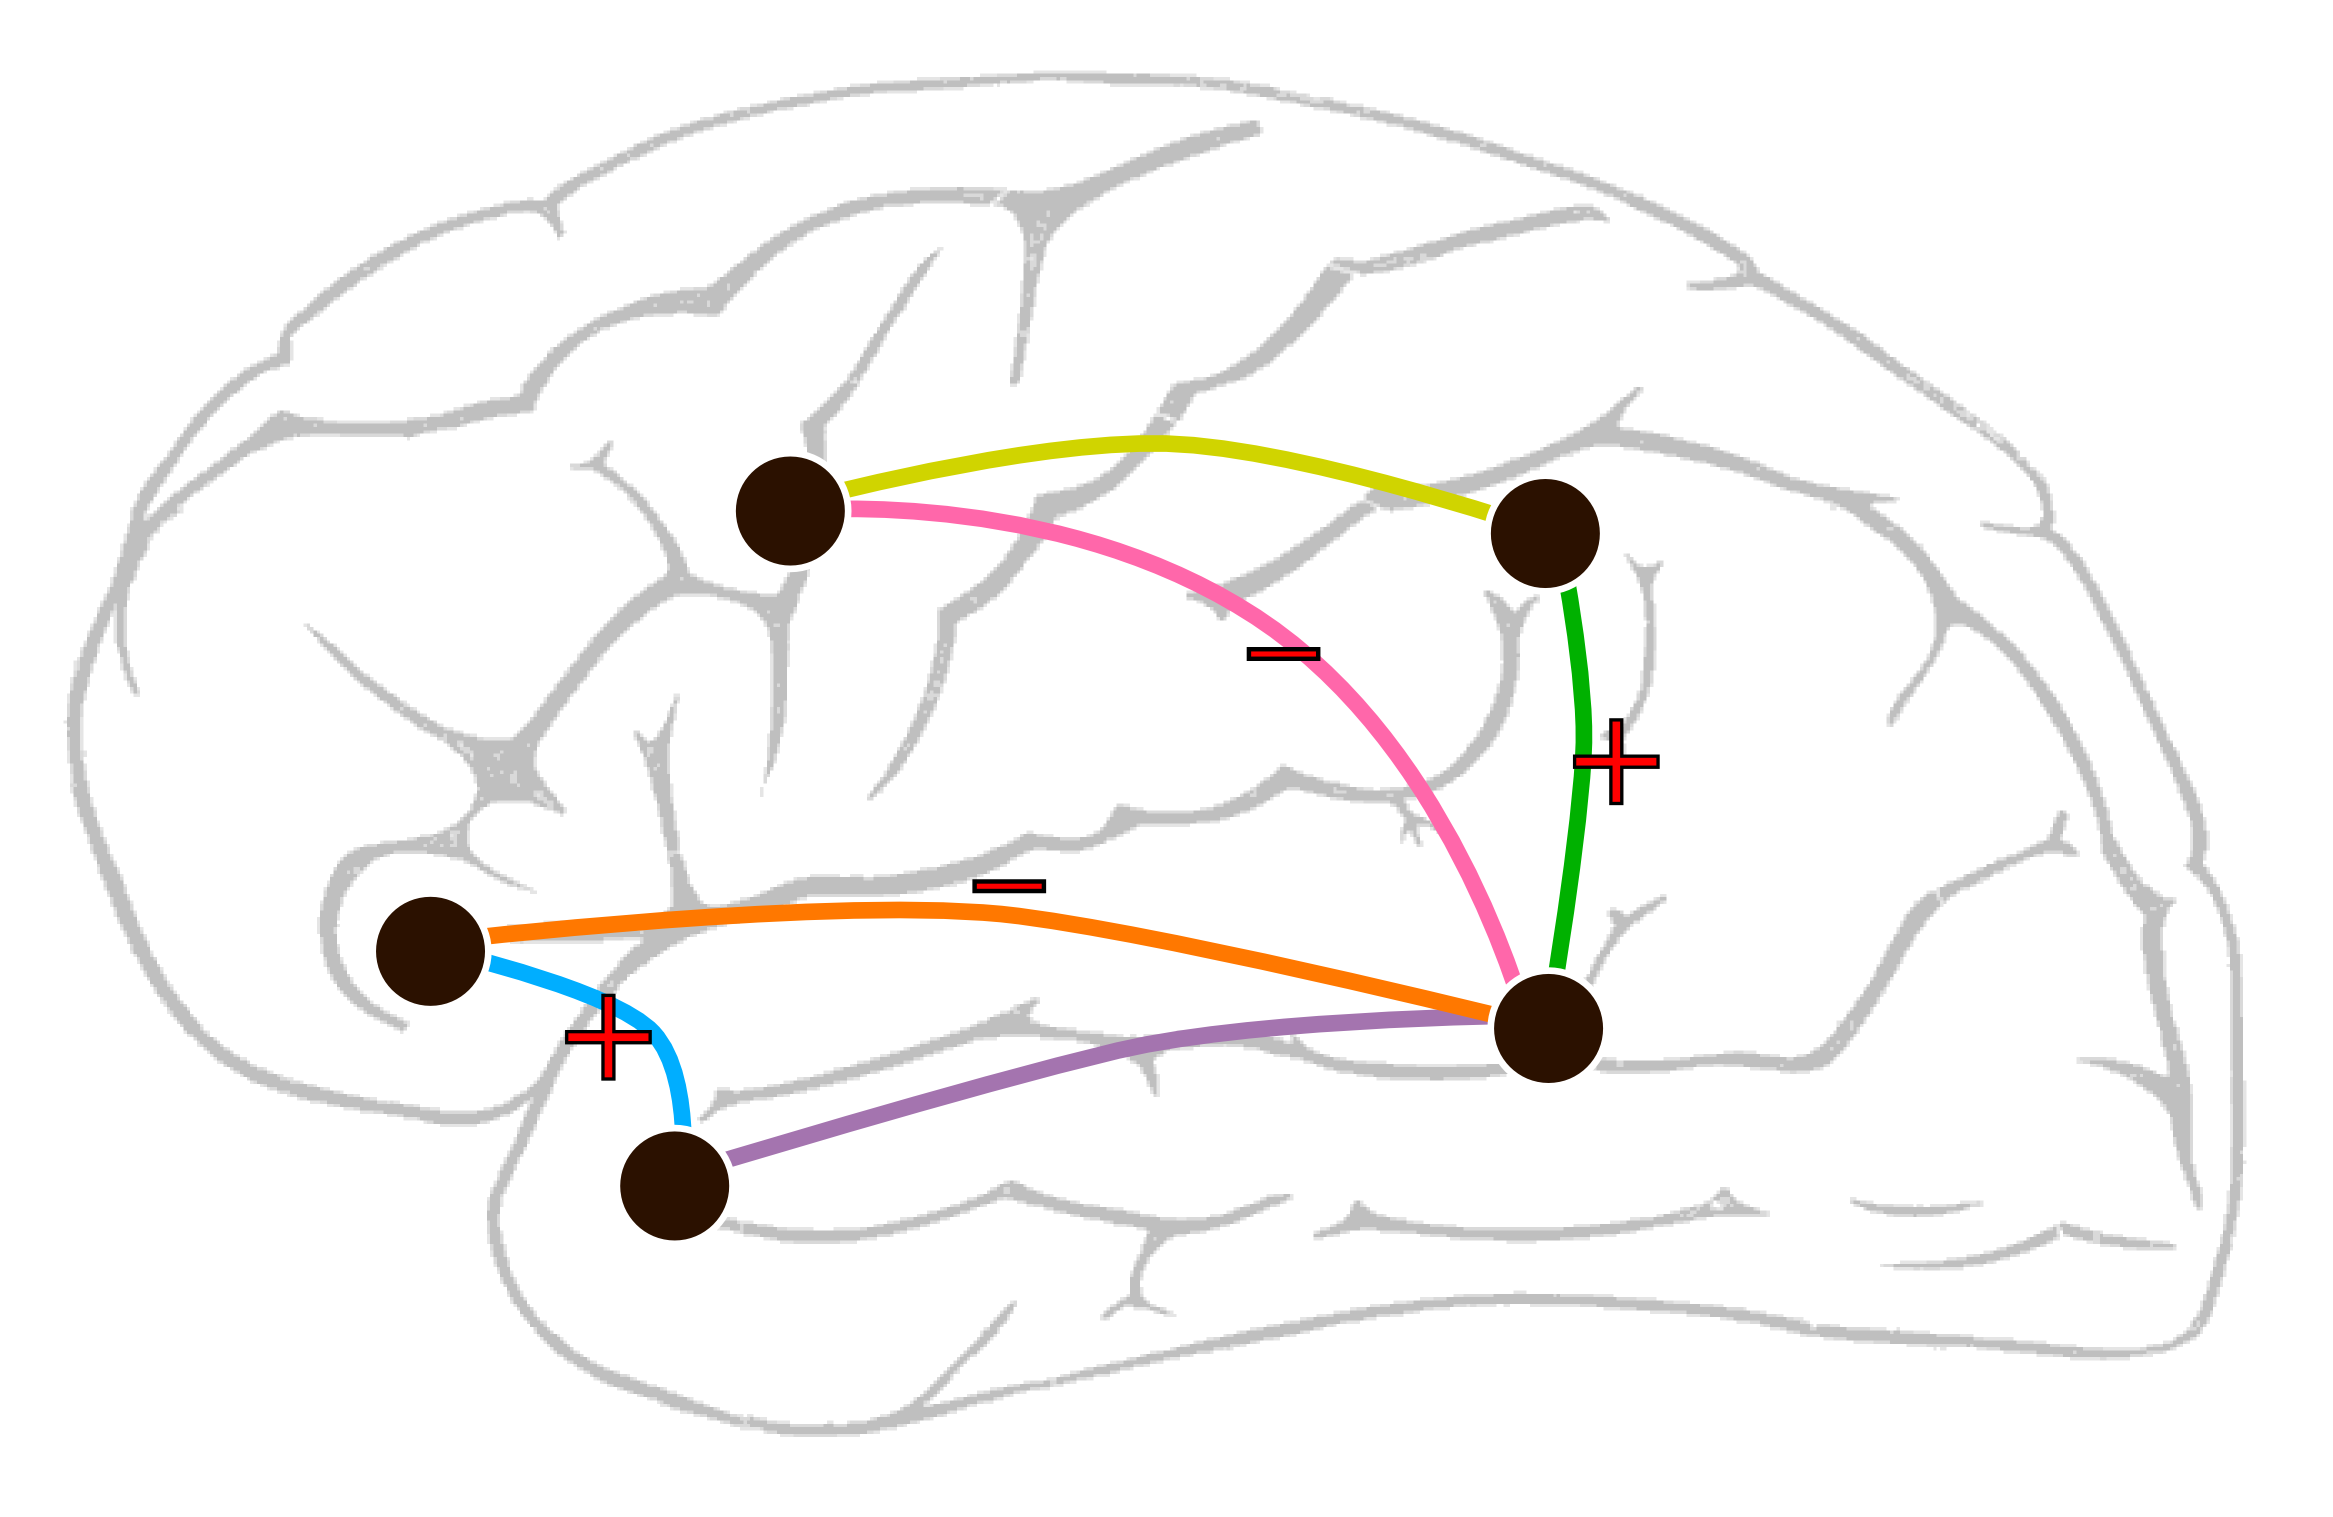
\includegraphics[width=0.45\linewidth]{figures/struct_diag2.png}
\end{tabular}
\caption{Stepwise multiple linear regression analysis examining performance in the subordinate context and tract averaged FA implicated all biological connections in the network: uncinate fasciculus (UNC), arcuate fasciculus (ARC), superior longitudinal fasciculus (SLF), inferior longitudinal fasciculus (ILF), inferior frontal-occipital fasciculus (IFO) and the arcuate fasciculus vertical (AFV). The coefficients for each structure are illustrated here. *Indicates an individually significant fiber tract ($p<0.05$).}
\label{fig:mlr_fa}
\end{center}
\end{figure}



\section{Functional Connectivity}
\label{appa}
\begin{table}[h]
\begin{center}
\tiny
\begin{tabular}{| l | r l | r l | r l |}
\hline
Regions & \multicolumn{2}{|c|}{Dominant} & \multicolumn{2}{|c|}{Neutral} & \multicolumn{2}{|c|}{Subordinate}\\
\hline
OFC $\leftrightarrow$ ATC &     (0.6) & $0.471 \pm 0.303$ &  (0.5) & $ 0.418 \pm 0.362$ &  (0.5) & $ 0.375 \pm 0.380$\\
ATC $\leftrightarrow$ PLTC &    (0.5) & $0.499 \pm 0.262$ &  (0.8) & $ 0.584 \pm 0.263$ &  (0.7) & $ 0.570 \pm 0.255$\\
OFC $\leftrightarrow$ PLTC &   (1.0) & $0.722 \pm 0.139$ &  (0.9) & $ 0.693 \pm 0.191$ &  (0.9) & $ 0.683 \pm 0.153$\\
PLTC $\leftrightarrow$ DLPFC & (1.0) & $0.701 \pm 0.010$ &  (0.9) & $ 0.671 \pm 0.164$ & (1.0)  & $ 0.686 \pm 0.126$\\
PLTC $\leftrightarrow$ IPC &    (0.7) & $0.488 \pm 0.287$ &  (0.6) & $ 0.484 \pm 0.300$ &  (0.6) & $ 0.493 \pm 0.236$\\
IPC $\leftrightarrow$ DLPFC &   (0.7) & $0.586 \pm 0.342$ &  (0.9) & $ 0.685 \pm 0.209$ &  (0.7) & $ 0.592 \pm 0.308$\\
\hline
\end{tabular}
\caption{Functional connectivity values between cortical ROIs with direct biological connections, as determined with DTI tractography. Cortical regions include orbital frontal (OFC), anterior temporal (ATC), posterior lateral temporal (PLTC), dorso-lateral prefrontal (DLFPC), and inferior partietal (IPC). The number in parentheses is the fraction of subjects that exhibited significant ($p < 0.05$) functional connectivity for that pair of regions. This is followed by the mean and standard deviation of the correlations for all subjects.}
\label{table:fcvalues}
\end{center}
\end{table}

\section{Fractional Anisotropy}
\label{appb}
\begin{table}[h]
\begin{center}
\begin{tabular}{| l | l |}
\hline
Structure & Average FA\\
\hline
Uncinate fasciculus & $ 0.397 \pm 0.092$\\
Inferior longitudinal fasciculus & $ 0.479 \pm 0.142$\\
Inferior fronto-occipital fasciculus & $ 0.646 \pm 0.122$\\
Arcuate fasciculus & $ 0.459 \pm 0.151$\\
Arcuate fasciculus (vertical) & $ 0.511 \pm 0.099$\\
Superior longitudinal fasciculus & $ 0.523 \pm 0.068$\\
\hline
\end{tabular}
\caption{Fractional anisotropy values in the white matter pathways that provide biological connectivity between the functional regions of interest.}
\label{table:connect}
\end{center}
\end{table}

